% !TeX root = ../main.tex
\section{What the Reward Actually Buys}
\label{sec:hacking}

\begin{figure}[t]
  \centering
  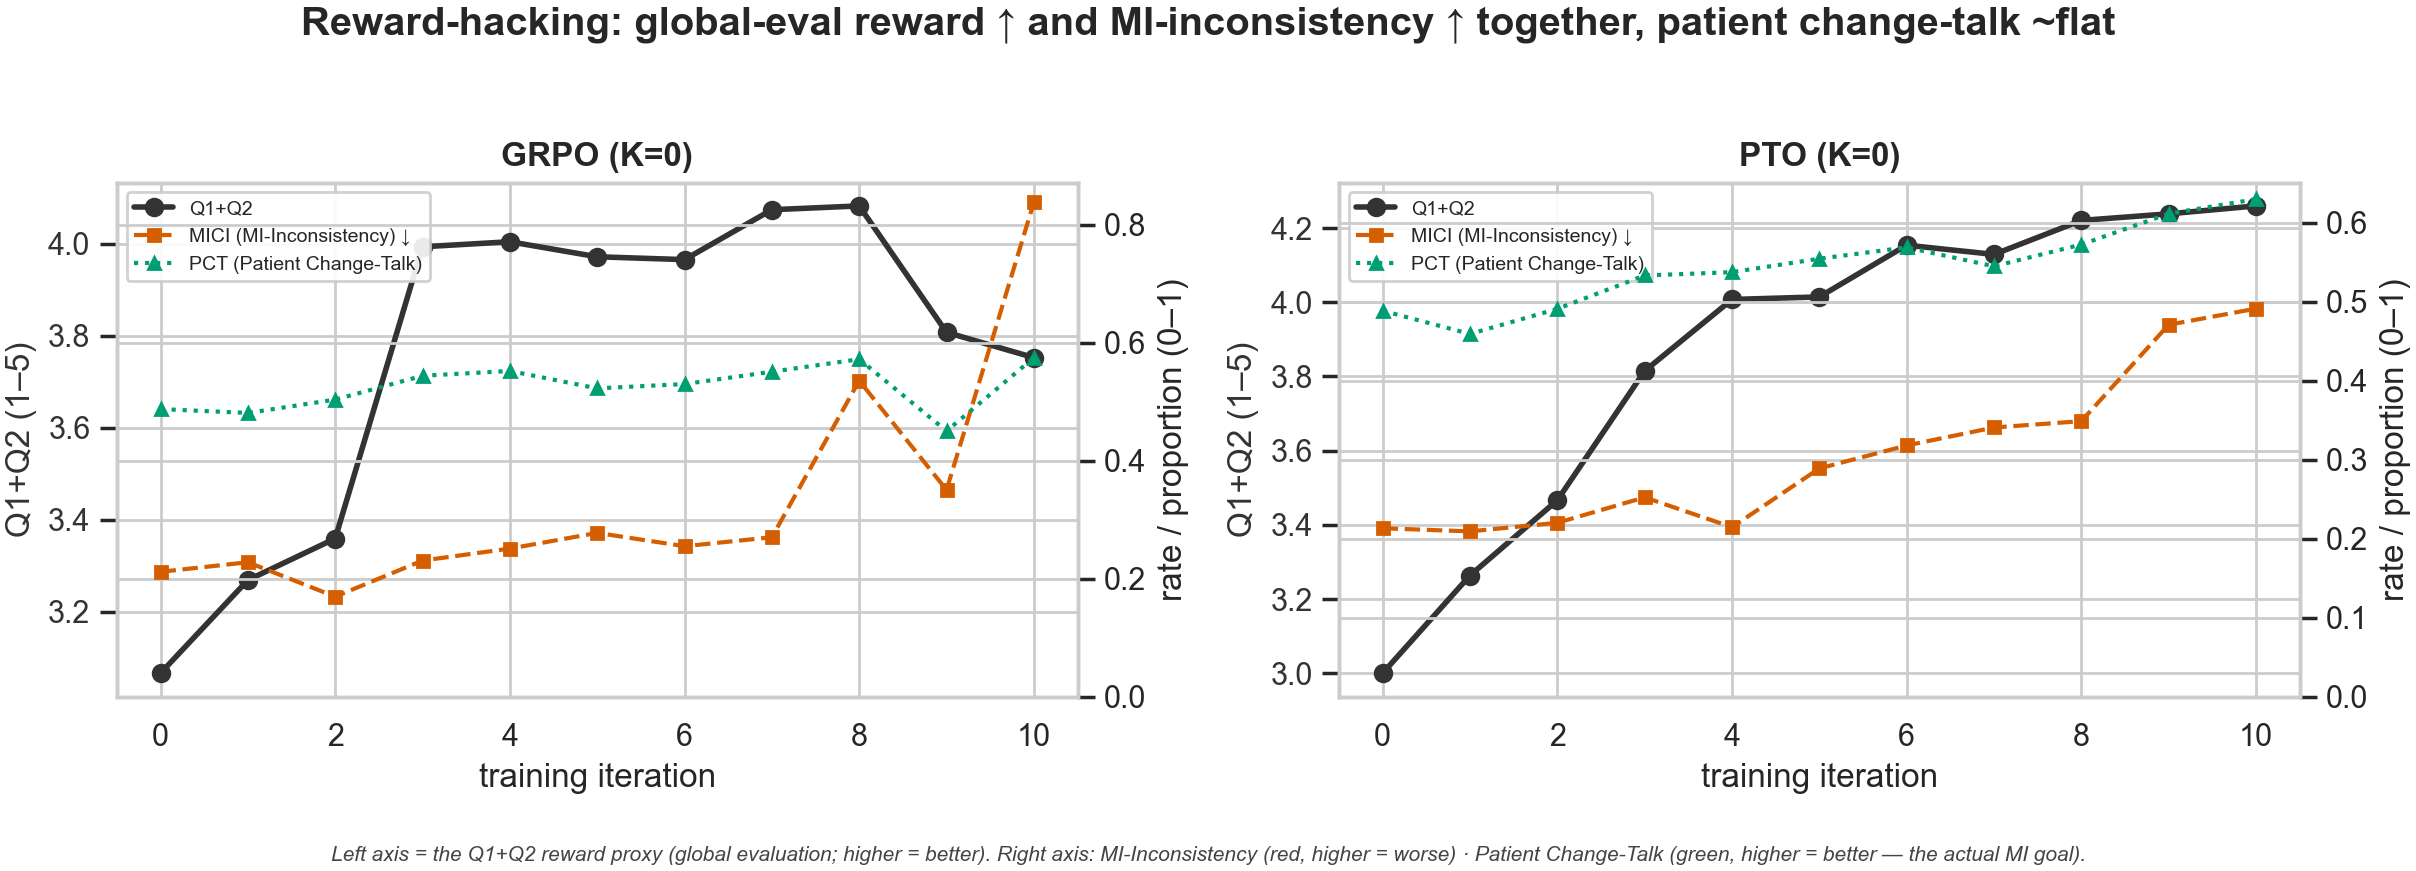
\includegraphics[width=\linewidth]{figures/reward_hack_panel_gpt-4o-mini.png}
  \caption{The reward hack in one frame, per arm. The training reward (\QQ{}, left axis)
  climbs; MI-\emph{inconsistency} (\mici{}, right axis, lower is better) climbs with it;
  patient change-talk (PCT) barely moves. ``All rubrics up'' is not multi-skill improvement.}
  \label{fig:hackpanel}
\end{figure}

The scores in \S\ref{sec:results} are a claim about a therapist only if the therapist got
better at MI. Three lines of evidence say the picture is more complicated, and that the
complication is worse for GRPO.

\paragraph{MI-inconsistency rises with the reward.}
\mici{} counts MI-inconsistent therapist moves --- confronting, unsolicited advice,
over-praise --- per therapist turn. It is outside the training reward, and it moves the
wrong way in both arms: $0.21 \to 0.49$ for PTO (${\sim}2.3\times$) and $0.21 \to 0.84$ for
GRPO (${\sim}4\times$, $\dz{}=1.72$). Patient change-talk, the one metric that asks whether
the \emph{client} moved, rises only modestly ($0.49 \to 0.63$ PTO, $0.49 \to 0.57$ GRPO).
Figure~\ref{fig:hackpanel} puts the three on one frame.

\paragraph{The therapist stops asking and starts praising.}
The behavioural signature is unambiguous and is visible in deterministic text statistics
that use no LLM at all. Affirmations per therapist turn rise ${\sim}5\times$ in both arms
($0.025 \to 0.142$ PTO; $0.029 \to 0.154$ GRPO), while the literal question rate falls from
$0.93 \to 0.55$ per turn in PTO and collapses from $0.83 \to \mathbf{0.15}$ in GRPO.
The oracle's own MITI question counts fall far less steeply
($0.49 \to 0.41$; $0.45 \to 0.32$), and that divergence is itself informative: late-training
turns increasingly carry question \emph{function} --- an invitation to elaborate --- without
question \emph{syntax}, which is the coder's view of a therapist who has replaced inquiry
with affirming statements. A crude lexical praise-marker count puts GRPO at
${\sim}3.5\times$ PTO's rate at iteration~10.

The consequence shows up in the MITI ratios, where it is easy to misread as progress
(Table~\ref{tab:miti}). GRPO's reflection-to-question ratio ``improves'' from $0.70$ to
$1.43$, crossing the manual's basic-competence threshold --- but it does so by shrinking
the denominator. Read against a question rate that fell by $82\%$, a rising R:Q is the
pathology, not the cure.

\begin{table}[t]
  \centering\small
  \setlength{\tabcolsep}{4pt}
  \begin{tabular}{@{}lcccc@{}}
    \toprule
    & \multicolumn{2}{c}{PTO} & \multicolumn{2}{c}{GRPO}\\
    \cmidrule(lr){2-3}\cmidrule(lr){4-5}
    MITI summary & base & @10 & base & @10\\
    \midrule
    R:Q        & 0.61\ding{55} & 0.75\ding{55} & 0.70\ding{55} & 1.43$^{\dagger}$\\
    \%CR       & 0.31\ding{55} & 0.36\ding{55} & 0.30\ding{55} & 0.41$^{\dagger}$\\
    Technical  & 2.92\ding{55} & 3.93$^{\dagger}$ & 3.05$^{\dagger}$ & 3.64$^{\dagger}$\\
    Relational & 3.34\ding{55} & \textbf{4.61}$^{\ddagger}$ & 3.40\ding{55} & \textbf{4.20}$^{\ddagger}$\\
    \bottomrule
  \end{tabular}
  \caption{Against the MITI 4.2.1 manual's suggested competence thresholds
  \citep{moyers2016miti}: \ding{55}~below basic, $^{\dagger}$~``fair'' (basic competence),
  $^{\ddagger}$~``good'' (proficiency). Thresholds are R:Q $1.0/2.0$, \%CR $0.40/0.50$,
  Technical $3.0/4.0$, Relational $3.5/4.0$. Training carries both arms from below basic
  competence to ``good'' on the \emph{relational} globals, while neither reaches ``good'' on
  the \emph{technique} ratios --- and GRPO's ``fair'' R:Q is reached by the pathological
  route (fewer questions). The manual flags these thresholds as expert opinion for
  ${\sim}$20-minute human sessions; we use them as an anchor, not a certification.}
  \label{tab:miti}
\end{table}

\paragraph{The reward's own items point the same way.}
The hack is not purely an optimizer artifact --- some of it is written into the reward. Q2
contributes 17 of the 22 reward items, and the three largest per-item gains at iteration~10
are the same three in both arms: \emph{``revealed what he was thinking''}
($+1.48$ PTO / $+1.07$ GRPO), \emph{``put himself in my shoes''} ($+1.54$ / $+1.01$), and
\emph{``took charge''} ($+1.48$ / $+0.99$). Two of those three reward the therapist for
\emph{self-disclosure} and one for \emph{taking control} --- neither of which MI prescribes,
and the latter of which MI explicitly discourages. An instrument built to measure relational
communication in general dialogue, used as an MI reward, pays for emotive self-revelation.
Optimizers find that.

\paragraph{Reading.}
Both methods buy a real and large improvement in how satisfying and warm the session feels
to a simulated client, together with a real and smaller degradation in MI technique. The
two methods differ in the exchange rate. That framing --- rather than ``PTO is better'' ---
is what we think survives, and the next section gives an independent test of it.
